%! Author = adnansiddiquei
%! Date = 13/12/2023

\subsection{Q3 - Dataset C}\label{subsec:dataset-c}
    \begin{figure}
    \centering
    \begin{subfigure}{0.9\textwidth}
        \centering
        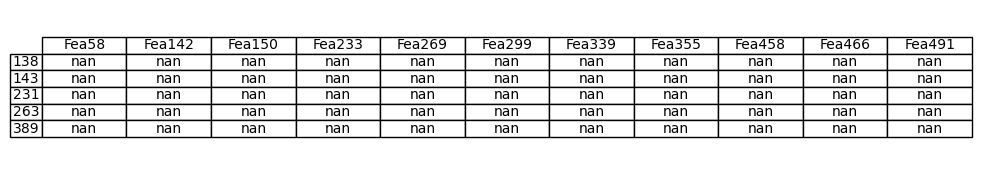
\includegraphics[width=1\textwidth]{./figures/q3a}
        \caption{The samples and features with missing data.}
        \label{fig:q3a}
    \end{subfigure}%
    \hfill
    \begin{subfigure}{0.9\textwidth}
        \centering
        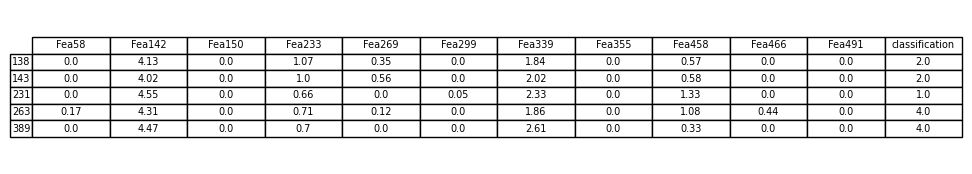
\includegraphics[width=1\textwidth]{./figures/q3c_1}
        \caption{The imputed data.}
        \label{fig:q3c}
    \end{subfigure}
    \caption{Samples and features with missing data, for the \inlinecode{C_MissingData.csv} dataset.}
    \label{fig:q3ac}
    \end{figure}

\subsubsection{Questions 3a and 3b}\label{subsubsec:q3ab}
    Figure \eqref{fig:q3a} displays features with missing values and corresponding samples.
    Several methods address missing data.
    Static imputation, a simple approach, replaces missing values in a feature with a constant value, like the feature's mean.
    Although computationally cost-effective, it may decrease variance and bias datasets with many missing values.
    Alternatively, model based imputation estimates missing values per sample using a suitable model.
    For example, the K Nearest Neighbours method imputes a feature's missing value using the mean of that value from
    the sample's K nearest neighbours.
    This approach can mitigate bias and maintain variance, but in high-dimensional data, it may lead to less meaningful
    nearest neighbours, as distances become less meaningful with increased dimensions \cite{bellman1957}.

    Multiple imputation involves using a probabilistic model to impute missing data several times, creating multiple datasets.
    These datasets can be analysed individually or their imputed values averaged.
    This method captures uncertainty in missing data, and is particularly useful when missing data is extensive.

\subsubsection{Question 3c}\label{subsubsec:q3c}
    \begin{figure}[htb]
    \centering
    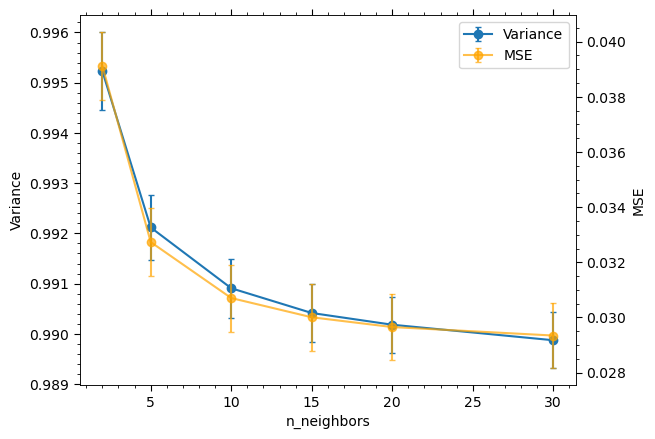
\includegraphics[width=0.9\textwidth]{./figures/q3c_optimise_knn_imputer}
    \caption{Variance and MSE of KNN imputed data, for different values of \inlinecode{n_neighbors}. The variance is shown as a
        percentage of the original dataset, and the MSE is the mean squared error of predicted values against the true
        values.}
    \label{fig:q3c_optimise_knn_imputer}
    \end{figure}

    \begin{figure}[htb]
    \centering
    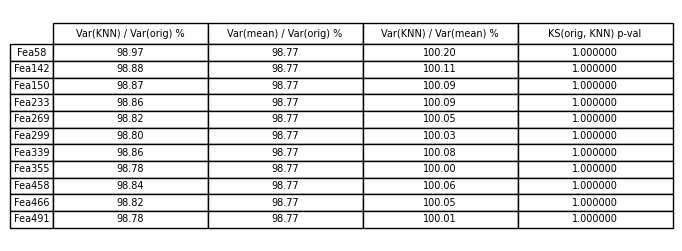
\includegraphics[width=0.9\textwidth]{./figures/q3c_2}
    \caption{This table compares feature variances post-imputation.
        Column 1 displays each feature's variance after KNN imputation, as a percentage of the original dataset.
        Column 2 does the same for mean imputation.
        Column 3 contrasts the values from columns 1 and 2.
        Column 4 presents the p-value from the Kolmogorov-Smirnov test, comparing the original and KNN imputed datasets.}
    \label{fig:q3c_2}
    \end{figure}

    Fig\eqref{fig:q3c_optimise_knn_imputer} depicts a simulation where data was removed and re-imputed using PCA and
    KNN to assess imputation accuracy at different \inlinecode{n_neighbors} values.
    This helped in selecting \inlinecode{n_neighbors=15} for KNN imputation, as larger \inlinecode{n_neighbors} values did not significantly
    improve accuracy (lower MSE).
    KNN combined with PCA mitigates the 'curse of dimensionality,' improving accuracy \cite{bellman1957} and aiding in
    identifying more meaningful neighbours.
    KNN is preferable for clustered datasets where distance-based methods are effective and it is expected that nearest
    neighbours share similar properties.

    Fig\eqref{fig:q3c} displays the data imputed with PCA and KNN.
    Fig\eqref{fig:q3c_2} indicates that this method largely preserved the original feature distributions.

\subsubsection{Question 3d and 3e}\label{subsubsec:q3de}
    \begin{figure}[htb]
    \centering
    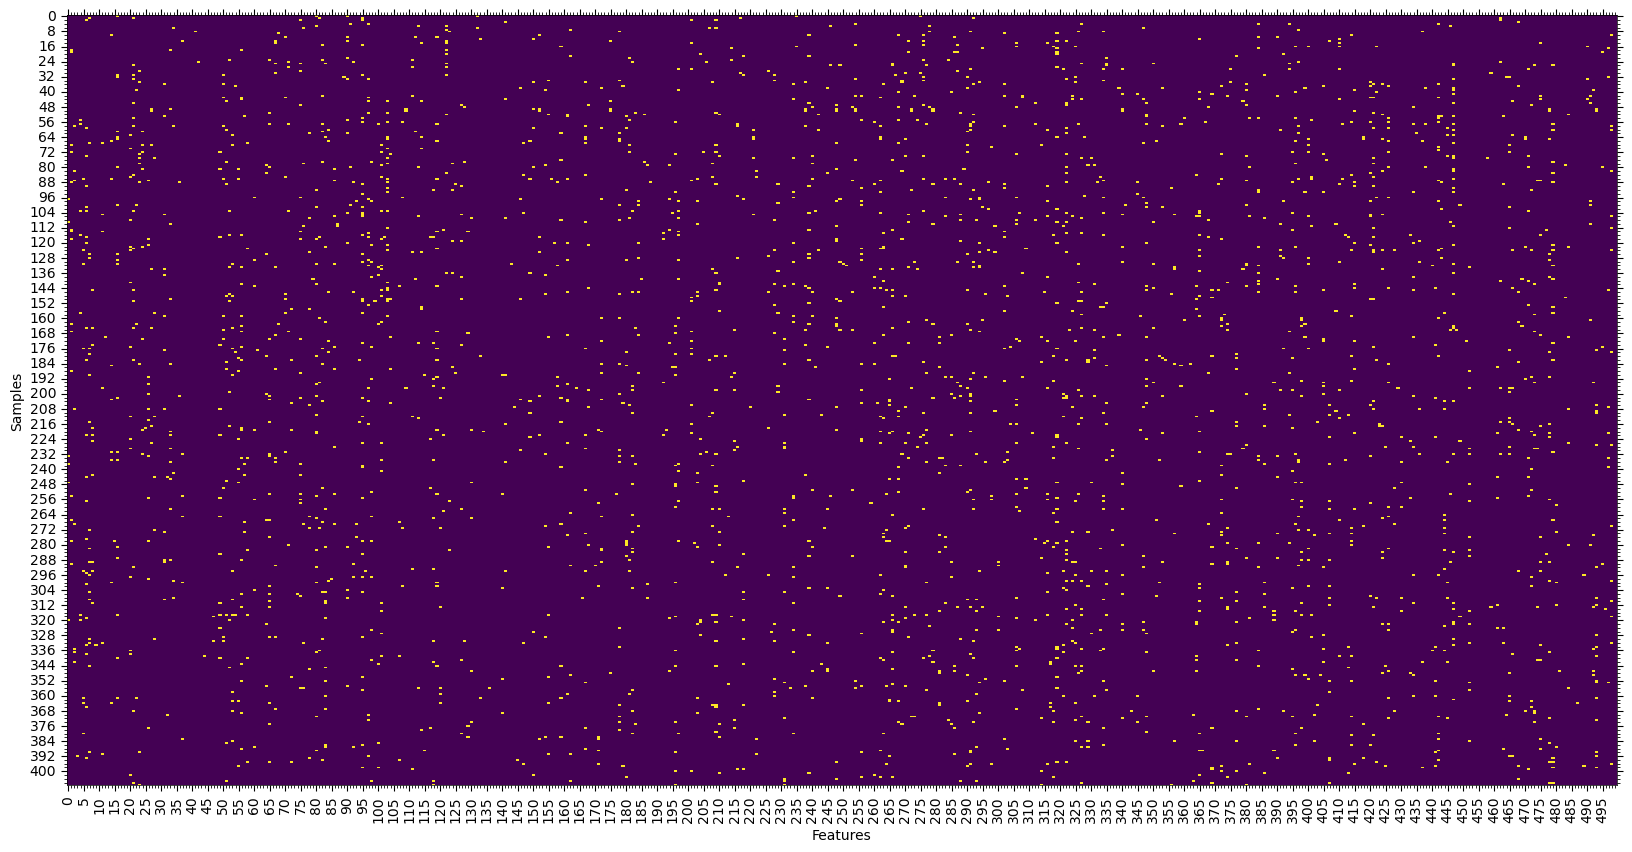
\includegraphics[width=1\textwidth]{./figures/q3d_heatmap}
    \caption{A heatmap of the outliers in the \inlinecode{C_MissingFeatures.csv} dataset. The orange marks indicate an
        outlier value, 2904 outlier values were identified.}
    \label{fig:q3d_heatmap}
    \end{figure}

    \begin{figure}[htb]
    \centering
    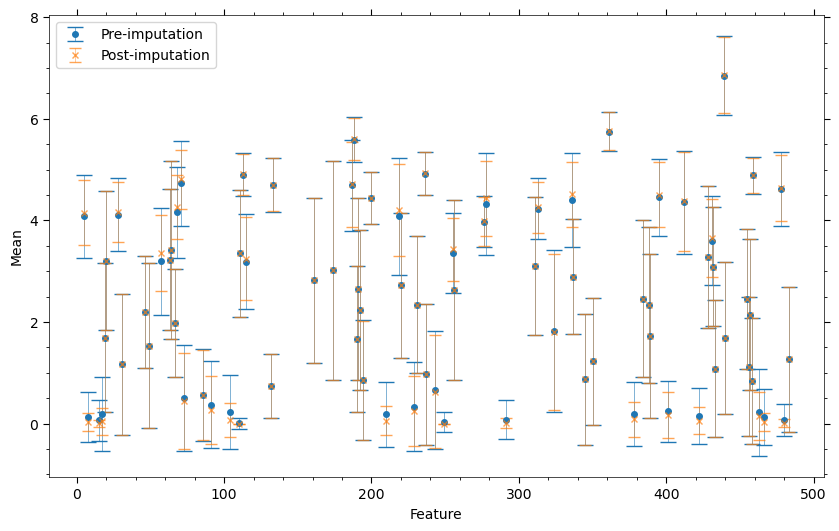
\includegraphics[width=0.9\textwidth]{./figures/q3e}
    \caption{The mean and standard deviation of the 81 most discriminative features in the original
        \inlinecode{C_MissingFeatures.csv} dataset, before and after outlier imputation.}
    \label{fig:q3e}
    \end{figure}

    Outliers were identified by standardising the data and identifying values over $3\sigma$ from the mean.
    Fig.\eqref{fig:q3d_heatmap} indicates uniformly distributed outliers across the dataset.

    These outliers were imputed using PCA and KNN, as in Question 3c, with the justification being identical to
    Question 3c.
    Outliers were iteratively removed, with re-standardisation and outlier detection after each iteration.
    The process iterated 8 times, stopping only after 0.27\% of the samples were outside $3\sigma$, aligning with normal
    distribution expectations.

    Fig.\eqref{fig:q3e} compares the mean and standard deviation of the 81 most discriminative features, before and after
    outlier imputation.
    Feature variance decreased post-imputation (as expected), more so for features with near-zero means, likely due to
    their sparsity and higher outlier likelihood.
